\scanpage{20}
\uline{Espace loc. modéré} Esp. \deleted{loc. cpct} \inserted{ind-modérés} dont la top. est \deleted{loc. cpcte} séparée, et tt point admet un \uline{voisinage} qui est \deleted{\unsure{esp.|cpt}} modéré (donc l'espace est loc. cpct), et tt pt admet un syst. fond. de voisinages modérés, et les parties compactes sont les parties contenues dans une partie modérée --- qui forment donc un antifiltre cofinal : celui des parties compactes.

Par exemple, par $(M10)$ $R$ est un espace $\mathrm{loc}^{\mathrm t}$ modéré, donc les $R^I$ aussi.

Les espaces loc. modérés \deleted{$\unsure{f}\ \operatorname{Esp}_{\mathrm{loc},\mathcal M_*}$} forment une sous-catégorie pleine $\operatorname{Esp}_{\mathrm{loc},\mathcal M_*}$ de $\underrightarrow{\operatorname{Esp}}_{\mathcal M_*}$, stable par $\varprojlim$ finies.

\margin{Dire qu'une partie compacte et \deleted{fermée} d'un espace modéré est modérée.}
\margin{\deleted{\unsure{loc.}}}
\figure{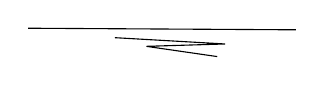
\begin{tikzpicture}\draw (0,0)--(3.4,-.02);\draw (1.1,-.12)--(2.5,-.2)--(1.5,-.23)--(2.4,-.36);\end{tikzpicture}}
\mspage{19}
